% Adjust these for the path of the theme and its graphics, relative to this file
%\usepackage{beamerthemeFalmouthGamesAcademy}
\usepackage{../../beamerthemeFalmouthGamesAcademy}
\usepackage{multimedia}
\graphicspath{ {../../} }

% Default language for code listings
\lstset{language=Python
}

% For strikethrough effect
\usepackage[normalem]{ulem}
\usepackage{wasysym}

\usepackage{pdfpages}

% http://www.texample.net/tikz/examples/state-machine/
\usetikzlibrary{arrows,automata}

\newcommand{\modulecode}{COMP260}\newcommand{\moduletitle}{Distributed Systems}\newcommand{\sessionnumber}{5}

\begin{document}
\title{\sessionnumber: Library Resources}
\subtitle{\modulecode: \moduletitle}

\frame{\titlepage} 

\begin{frame}{These slides are online...}
	\begin{center}
		On the ``BSc Computing for Games Course Page'', under ``COMP Enhancement (Year 1)''
	\end{center}
\end{frame}

\begin{frame}{Learning objectives}
	By the end of this session, you should be able to:
	\begin{itemize}
		\item \textbf{Explain} what constitutes a ``scholarly source'';
		\item \textbf{Determine} whether a given source is appropriate to use in academic work;
		\item \textbf{Use} physical and electronic library resources to access scholarly sources;
		\item \textbf{Write} correctly formatted references in IEEE format
	\end{itemize}
\end{frame}

\part{Scholarly literature}
\frame{\partpage}

\begin{frame}{Scholarly work}
	\begin{itemize}
		\pause\item What is a ``scholarly'' work?
		\pause\item How do we know if something is scholarly?
	\end{itemize}
\end{frame}

\usetikzlibrary{shapes,arrows,intersections}
\usetikzlibrary{matrix,fit,calc,trees,positioning,arrows,chains,shapes.geometric,shapes}

\begin{frame}{Pyramid of sources}
	\centering
	\begin{tikzpicture}
	\coordinate (A) at (-4.5,0) {};
	\coordinate (B) at ( 4.5,0) {};
	\coordinate (C) at (0,5*1.2) {};
	\path[name path=AC,draw=none] (A) -- (C);
	\path[name path=BC,draw=none] (B) -- (C);
	\iftoggle{printable}{
		\filldraw[draw=Purple, ultra thick,fill=Purple!10!White] (A) -- (B) -- (C) -- cycle ;
	}{ % else
		\filldraw[draw=Purple, ultra thick,fill=Purple!10!Black] (A) -- (B) -- (C) -- cycle ;
	}	

	\foreach \y/\A in {4.5/{Scholarly journals and conference proceedings},
					   4.0/{Scholarly books and book chapters},
					   3.5/{Masters and PhD theses},
					   3.0/{Government documents, trade books and white papers},
					   2.5/{Specialised magazines},
					   2.0/{Pre-print papers (e.g.\ arXiv)},
					   1.5/{General interest books, magazines and newspapers},
					   1.0/{General encyclop\ae dias},
					   0.5/{Websites, blogs, Wikipedia},
					   0.0/{Online discussion boards, personal communications}
					} {
		\pause
		\path[draw=none, very thick, dashed, name path=horiz] (A|-0,\y*1.2) -- (B|-0,\y*1.2);
		\draw[draw=Purple, very thick, dashed, 
			  name intersections={of=AC and horiz,by=P},
			  name intersections={of=BC and horiz,by=Q}] (P) -- (Q)
			  %node[midway,above,font=\bfseries\scshape,color=red!60!Brown] {\A};
			  node[midway,above] {\A};
	}
	\end{tikzpicture}
\end{frame}

\begin{frame}{Appropriateness of sources}
	\pause It is important to question the \textbf{appropriateness} of sources you use in academic work
	\begin{itemize}
		\pause\item \textbf{Validity}: Are claims based upon a correct interpretation of the evidence?
		\pause\item \textbf{Rigor}: Was the method of collecting evidence appropriate to ensure 
			comprehensive coverage while also avoiding bias?
	\end{itemize}
\end{frame}

\begin{frame}{Appropriateness of sources}
	\begin{itemize}
		\pause\item \textbf{Reliability}: has the claim been replicated, or at least reviewed, by other academics?
		\pause\item \textbf{Authoritativeness}: do we know who the author is?
			Does the author have enough experience in the field to present a fair and balanced argument?
		\pause\item \textbf{Venue}: Is the publisher reputable and free of undue editorial influences?
	\end{itemize}
\end{frame}

\begin{frame}{Appropriateness of sources}
	\pause There are of course exceptions where sources are presented as \textbf{artefacts} and/or \textbf{archives}:
	\begin{itemize}
		\pause\item Citing a newspaper as evidence for a claim based on the reception of a new technology
		\pause\item Citing a manufacturer's technical manual when describing a technical feature of a platform
		\pause\item Citing a Reddit post by a well-known industry figure as evidence for expert opinion
	\end{itemize}
	\pause The \textbf{way} in which sources are \textbf{used} is therefore important
\end{frame}

\part{Library resources}
\frame{\partpage}

\begin{frame}{Library catalogue}
	\begin{center}
		\url{http://library.fxplus.ac.uk/}
	\end{center}
\end{frame}

\begin{frame}{Web proxy}
	Insert \texttt{.ezproxy.falmouth.ac.uk} at the end of the \textbf{domain name}
		(before the \texttt{/})
	\pause
	\begin{center}
		\texttt{http://www.example.com/example/page.html}
		
		\pause $\downarrow$
		
		\texttt{http://www.example.com\uline{.ezproxy.falmouth.ac.uk}/ example/page.html}
	\end{center}
\end{frame}

\begin{frame}{ACM Digital Library}
	\begin{center}
		\small\url{http://dl.acm.org.ezproxy.falmouth.ac.uk/}
	\end{center}
\end{frame}

\begin{frame}{IEEE Xplore}
	\begin{center}
		\small\url{http://ieeexplore.ieee.org.ezproxy.falmouth.ac.uk/}
	\end{center}
\end{frame}

\begin{frame}{GDC Vault}
	\begin{center}
		\small\url{http://www.gdcvault.com.ezproxy.falmouth.ac.uk/}
		
		\vspace{2ex}
		
		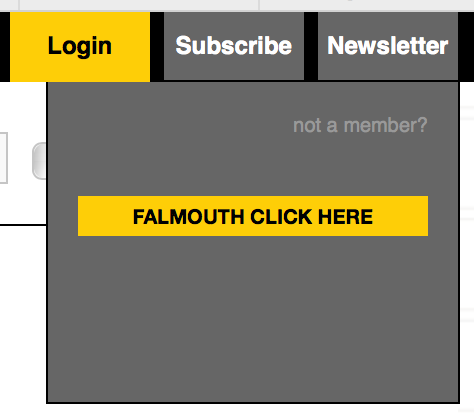
\includegraphics[width=0.4\textwidth]{gdc_login}
	\end{center}
\end{frame}

\begin{frame}{Ethics of paywalls}
	\begin{itemize}
		\pause\item Is it ethical for publishers to charge for access to publicly-funded academic research?
		\pause\item Many journals offer free \textbf{open access}
			\begin{itemize}
				\pause\item Some high quality, some low quality...
			\end{itemize}
		\pause\item Many authors put papers on their \textbf{personal websites}
			\begin{itemize}
				\pause\item Some publishers allow this, others turn a blind eye
			\end{itemize}
		\pause\item Sites like \textbf{sci-hub} aim to be a ``Pirate Bay for papers''
	\end{itemize}
\end{frame}

\part{Referencing}
\frame{\partpage}

\begin{frame}{Which referencing style?}
	\begin{itemize}
		\pause\item Many different referencing styles exist
		\pause\item Most Falmouth courses use \textbf{Harvard} style
		\pause\item In Computing we tend to prefer \textbf{IEEE} style
		\pause\item If assignments specify which one to use then use it
		\pause\item Otherwise choose whichever you prefer --- just be \textbf{consistent}
		\pause\item Tools like BibTeX make it easy to switch styles
	\end{itemize}
\end{frame}

\begin{frame}{Direct quotations}
	\begin{itemize}
		\pause\item \textbf{THIS IS IMPORTANT:} \#1 source of alleged academic misconduct cases for the Research Journal!
		\pause\item If you are directly quoting a source, you must make it \textbf{very clear} that this is the case
		\pause\item Common convention is to use \textbf{quotation marks and italics}, with a citation straight after ---
			\textit{``To be or not to be, that is the question''} [Shakespeare 1604]
		\pause\item Direct quotations are generally bad style in technical writing --- better to rephrase, summarise, synthesise key points
		\pause\item Most written assignments at Falmouth are passed through TurnItIn --- plagiarism \textbf{will} be detected!
	\end{itemize}
\end{frame}

\begin{frame}{IEEE referencing style}
	\begin{center}
		\small\url{https://ieeeauthorcenter.ieee.org/wp-content/uploads/IEEE-Reference-Guide.pdf}
	\end{center}
\end{frame}

\begin{frame}{Harvard referencing style}
	\begin{center}
		\small\url{https://studyhub.fxplus.ac.uk/study-guides/referencing/harvard-referencing-falmouth-university}
	\end{center}
\end{frame}

\begin{frame}{BibTeX entry types}
	\begin{center}
		\small\url{https://en.wikibooks.org/wiki/LaTeX/Bibliography_Management\#BibTeX}
	\end{center}
\end{frame}

\begin{frame}{Writing BibTeX entries}
	\begin{itemize}
		\pause\item Some websites provide pre-written BibTeX entries for papers
		\pause\item Beware of copying and pasting these as they are often incomplete, incorrectly formatted or just wrong!
		\pause\item You must \textbf{always} check your bibliography in the compiled PDF and fix any errors
		\pause\item You \textbf{will} lose marks on your written assignments otherwise!
	\end{itemize}
\end{frame}



\end{document}
